\chapter{\hisparc Network}
\label{ch:network}

Science Park air shower reconstructions...


\subsection{Shower reconstruction with multiple stations}

% Similar direction reconstruction algorithm as used for single station.
With the combined measurement data from multiple stations a more accurate reconstruction is possible. The distances between the detection points are larger while the timing accuracy remains excellent. The reconstruction algorithm needs to take into account the different relative altitudes of the detectors, since these are no longer all at the same altitudes \cite{steijger2012direction}. Note that for some stations (e.g. 507 and 1009) the detectors are also not all at the same altitude, but that is very rare. The Cartesian approach is used for 3D reconstruction of the shower direction \cite{montanus2015direction}

\begin{equation}
    \label{eq:direction3dflat}
    \begin{split}
        \phi &= \arctan \left(\frac{(\mathbf{u} \times \mathbf{v})_y \pm v_y \sqrt{v^2-u^2}}{(\mathbf{u} \times \mathbf{v})_x \pm v_x \sqrt{v^2-u^2}}\right) \ , \\
        \theta & = \arccos \left( \frac{(\mathbf{u} \times \mathbf{v})_z \pm v_z \sqrt{v^2-u^2}}{v^2}\right) \ .
    \end{split}
\end{equation}

Where ....[explain terms].

% At large core distances the curvature of the shower front should be taken into account.
Moreover, the curvature and rise time of the shower front play a big role and need to be accounted for in the reconstruction.

% For a large event should arrival times in each detector be used or station average density and average/first arrival time?
For stations separated by large distances the reconstruction can be performed using data from all individual detectors in each station or by using a station average. It depends on the used reconstruction algorithm what the best choice will be. In case of using the first arrival time from all detectors at the station arrival time will provide better results for a reconstruction assuming a flat shower front. In the case of a shaped shower front the reconstruction should take into account the probability of detection and thus the most likely arrival times. For arrival direction reconstruction using a shaped shower front the shower axis (core) location must be known. In \cref{fig:angle_between_501_minn16_510} reconstruction accuracy using the individual detector arrival times is compared to a reconstruction using station averages (or first?).

\begin{figure}
    \centering
    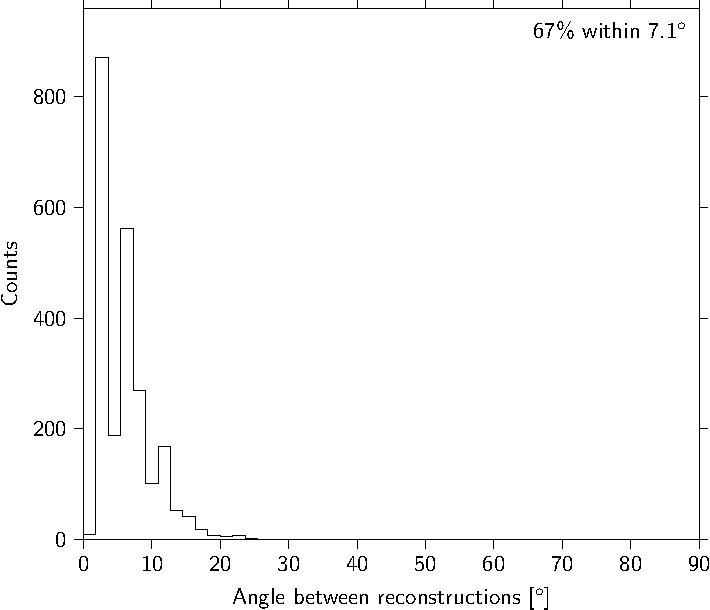
\includegraphics[width=0.6\textwidth]
                    {plots/cluster/angle_between_501_minn16_510}
    \caption{(placeholder plot, not data mentioned in caption) Distance between reconstructions when using average/first arrival time, versus simulation input. Using separate detectors should hold more information, but the reconstruction algorithm should be aware (using curved or flat reconstruction?)}
    \label{fig:angle_between_501_minn16_510}
\end{figure}


